\begin{center}

\includegraphics[width=0.6\textwidth]{content/3/chapter6/images/15.png}\\
Cippi directs the train
\end{center}

Semaphores are a synchronization mechanism used to control concurrent access to a shared resource. A counting semaphore is a special semaphore that has a counter that is bigger than zero. The counter is initialized in the constructor. Acquiring the semaphore decreases the counter and releasing the semaphore increases the counter. If a thread tries to acquire the semaphore when the counter is zero, the thread will block until another thread increments the counter by releasing the semaphore.


\begin{tcolorbox}[breakable,enhanced jigsaw,colback=blue!5!white,colframe=blue!75!black,title={Edsger W. Dijkstra invented Semaphores}]
	
The Dutch computer scientist \href{https://en.wikipedia.org/wiki/Edsger_W._Dijkstra}{Edsger W. Dijkstra} presented in 1965 the concept of a semaphore. A semaphore is a data structure with a queue and a counter. The counter is initialized to a value equal to or greater than zero. It supports the two operations wait and signal. Operation wait acquires the semaphore and decreases the counter. It blocks the thread from acquiring the semaphore if the counter is zero. Operation signal releases the semaphore and increases the counter. Blocked threads are added to the queue to avoid \href{https://en.wikipedia.org/wiki/Starvation_(computer_science)}{starvation}.

Originally, a semaphore was a railway signal.
	
\end{tcolorbox}

\begin{center}
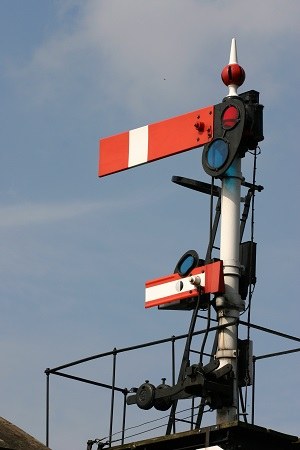
\includegraphics[width=0.6\textwidth]{content/3/chapter6/images/16.png}\\
Semaphore
\end{center}

The original uploader was AmosWolfe at English Wikipedia. - \href{https://commons.wikimedia.org/w/index.php?curid=1972304}{Transferred from en.wikipedia to Commons., CC BY 2.0,}

C++20 supports a std::binary\_semaphore, which is an alias for a std::counting\_semaphore<1>. In this case, the least maximal value is 1. std::binary\_semaphores can be used to implement \href{https://en.cppreference.com/w/cpp/named_req/BasicLockable}{locks}.

\begin{lstlisting}[style=styleCXX]
using binary_semaphore = std::counting_semaphore<1>;
\end{lstlisting}

In contrast to a std::mutex, a std::counting\_semaphore is not bound to a thread. This means that the acquire and release of a semaphore call can happen on different threads. The following table presents the interface of a std::counting\_semaphore.

\begin{center}
Member functions of a std::counting\_semaphore sem
\end{center}

\begin{table}[H]
\centering
\begin{tabular}{ll}
\textbf{Member function} & \textbf{Description}                                                       \\ \hline
sem.max() (static)       & Returns the maximum value of the counter.                                  \\
sem.release(upd = 1)             & Increases counter by upd and subsequently unblocks threads acquiring the semaphore sem.  \\
sem.acquire()            & Decrements the counter by 1 or blocks until the counter is greater than 0. \\
sem.try\_acquire()       & Tries to decrement the counter by 1 if it is greater than 0.               \\
sem.try\_acquire\_for(relTime)   & Tries to decrement the counter by 1 or blocks for at most relTime if the counter is 0.   \\
sem.try\_acquire\_until(absTime) & Tries to decrement the counter by 1 or blocks at most until absTime if the counter is 0.
\end{tabular}
\end{table}

The constructor call std::counting\_semaphore<10> sem(5) creates a semaphore sem with an at least maximal value of 10 and a counter of 5. The call sem.max() returns the least maximal value. sem.try\_aquire\_for(relTime) needs a \href{https://en.cppreference.com/w/cpp/chrono/duration}{time duration}; the member function sem.try\_acquire\_until(absTime) needs a \href{https://en.cppreference.com/w/cpp/chrono/time_point}{time point}. The three calls sem.try\_acquire, sem.try\_acquire\_for, and sem.try\_acquire\_until and return a boolean indicating the success of the calls.

Semaphores are typically used in sender-receiver workflows. For example, initializing the semaphore sem with 0 will block the receiver’s sem.acquire() call until the sender calls sem.release(). Consequently, the receiver waits for the notification of the sender. The previous program of onetime synchronization of threads can easily be reimplemented using semaphores.

\hspace*{\fill} \\ %插入空行
\noindent
Thread synchronization with a std::counting\_semaphore
\begin{lstlisting}[style=styleCXX]
// threadSynchronizationSemaphore.cpp

#include <iostream>
#include <semaphore>
#include <thread>
#include <vector>

std::vector<int> myVec{};

std::counting_semaphore<1> prepareSignal(0);

void prepareWork() {

	myVec.insert(myVec.end(), {0, 1, 0, 3});
	std::cout << "Sender: Data prepared." << '\n';
	prepareSignal.release();
}

void completeWork() {

	std::cout << "Waiter: Waiting for data." << '\n';
	prepareSignal.acquire();
	myVec[2] = 2;
	std::cout << "Waiter: Complete the work." << '\n';
	for (auto i: myVec) std::cout << i << " ";
	std::cout << '\n';

}

int main() {

	std::cout << '\n';
	
	std::thread t1(prepareWork);
	std::thread t2(completeWork);
	
	t1.join();
	t2.join();
	
	std::cout << '\n';

}
\end{lstlisting}

The std::counting\_semaphore prepareSignal (line 10) can have the values 0 and 1. In the concrete example, it’s initialized with 0 (line 10). This means, that the call prepareSignal.release() sets the value to 1 (line 16) and unblocks the call prepareSignal.acquire() (line 22).

\begin{center}
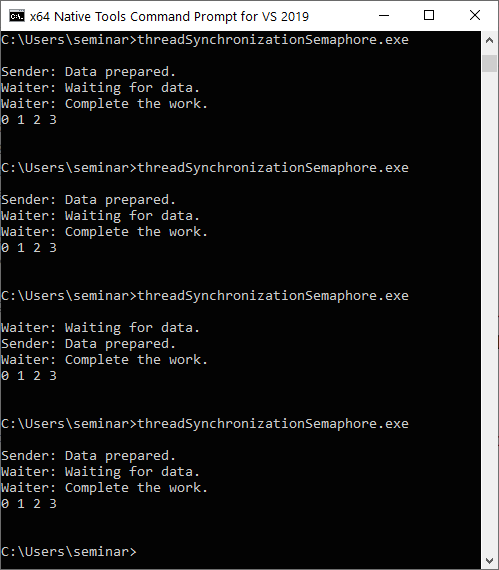
\includegraphics[width=0.6\textwidth]{content/3/chapter6/images/17.png}\\
Thread synchronization with semaphores
\end{center}

\begin{tcolorbox}[breakable,enhanced jigsaw,colback=mygreen!5!white,colframe=mygreen!75!black,title={Distilled Information}]
	
\begin{itemize}
\item 
Semaphores are a synchronization mechanism used to control concurrent access to a shared resource.

\item 
A counting semaphore in C++20 has a counter. Acquiring the semaphore decreases the counter and releasing the semaphore increases the counter. If a thread tries to acquire the semaphore when the counter is zero, the thread will block until another thread increments the counter by releasing the semaphore.
\end{itemize}
	
\end{tcolorbox}


















